\chapter{Experiment 2}
\label{exp2.0}
\lhead{Chapter 4. \emph{Experiment 2}} 

\section{Introduction}

In the previous chapter, we found evidence that the spatial encoding of the reach action target is influenced by the multi-modal nature of sensory information about the body-part in proximity to the target, with increased accuracy when the nature of this information is multi-modal, as compared to uni-sensory information. What does the multi-modal sensory information regarding the body imply? According to \citeauthor{ataria2021body}, signals from multiple sources like vision and proprioception are integrated to construct a representation of the body (\textit{body schema}, which specifies certain parameters like the position of the body part. Thus, one of the functions of multi-sensory integration is to compute reliable estimates of the location of the body part, by integrating the estimates provided by uni-sensory cues on the basis of its reliability and the relevance attributed to the particular modality \citep{limanowski2016integration, noel2018peri, kording2007causal, van1999integration}. Thus, it seems that this mechanism of multi-sensory integration which specifies the position of the body-part may underlie the spatial encoding of the target of reach action which is located in its proximity.

Generally, vision and proprioception provide congruent estimates about the position of the body. However, inducing discrepancy between the estimates provided by vision and proprioception allow us to probe further into proximal body-part multi-sensory integration mechanism underlying the spatial encoding of target. Therefore, in the following experiment, we manipulated the spatially discrepancy between the actual position of the non-action target proximal hand and its visual input, by spatially displacing the visually rendered hand in an Immersive Virtual Reality environment. The objective of this experiment was to understand how the target location estimation in reach action is affected by the spatial discrepancy between the estimate provided by proprioception and vision about the proximal body-part location. Specifically, we aimed to test the hypothesis that congruency between visual and proprioceptive estimates of proximal body-part location will lead to more accurate encoding of the spatial information of the target. We also aimed to understand how the differences in proximity to the body-part with incongruent estimates from visuo-proprioceptive inputs affects the target location estimation. 


%What is the location of my hand? The answer to this question is provided by inputs from multiple sensory modalities like vision and proprioception. Visual and proprioceptive information is integrated to infer an estimate regarding the location of the hand ~\citep{van1999integration}. Generally, vision and proprioception provide congruent estimates about the location of the body. However, inducing discrepancy between the estimates provided by vision and proprioception through experimental manipulation allows us to understand how the integration between the two modalities affects the representation of the target of the reach action.

%In the following experiment, we manipulated spatial discrepancy between the actual position of the hand and the visual input of the task-irrelevant hand, by spatially displacing the visually rendered hand in an Immersive Virtual Reality environment. The objective of this experiment was to understand how the target location estimation is affected by the spatial discrepancy induced between the estimate provided by proprioception and vision of the hand. We expected that reach error will be lowest in the condition where vision and proprioception are congruent. However, for visuo-proprioceptive incongruent conditions, we hypothesized that the way visuo-proprioceptive discrepancy affects the reach error is dependent upon the distance between the target and the non-action hand. 

\section{Method}

\subsection{Participants}
Nineteen right-handed subjects(2 Females, Mean age = 22.68, Range = 18-33) were recruited to participate in the experiment. All participants reported normal or corrected to normal vision. They were naive to the purpose of the experiment and the experimental procedure, and had provided written consent to participate in the study according to the norms approved by the Institute Ethics Committee (IEC) of Indian Institute of Technology, Kanpur. 

\subsection{Materials and Apparatus}
The participants sat across a table with surface area dimensions of 120cm x 50cm. Two coin-shaped docks (2.5 cm diameter) were attached to the table with a distance of 46 cm between them at the center of the table. A cylindrical barrier of 2.5cm height was attached around the right dock. The participant sat with their arms resting comfortably on the table, with the right and left docks serving as resting positions for the right and left index fingers respectively. Hand motion and position was tracked with Ultraleap Leap Motion Controller. The virtual reality environment was displayed on Oculus Rift S Head-mounted Display, and developed using Unity Game Engine. The virtual scene consisted of a virtual table situated in a black room. The virtual table was spatially aligned to the physical table at which the participant sat. The target of the reach was a red dot of 0.5cm in diameter. 

\subsection{Procedure}

The experiment began with a calibration session, similar to the session performed in Experiment 1 (Refer Chapter \ref{exp1}). The experiment consisted of 5 Experimental blocks which were interleaved with filler blocks. For the experimental blocks, the participants were instructed to place their left hand on the dock, whereas for the filler blocks, the left hand was placed on the lap. The experimental blocks differed in the position at which the left hand was rendered visually in the virtual scene. The visual rendering of the left hand, henceforth termed as the visual hand, was positioned at five locations - congruent to the left hand placed at the left dock (henceforth termed as the proprioceptive hand), 5.75cm, and 11.50cm to the right of proprioceptive hand, and 5.75cm and 11.50cm to the left of the proprioceptive hand. The order of the experimental blocks was counterbalanced across participants using Latin Square counterbalancing design. 

\begin{figure}
\centering       
    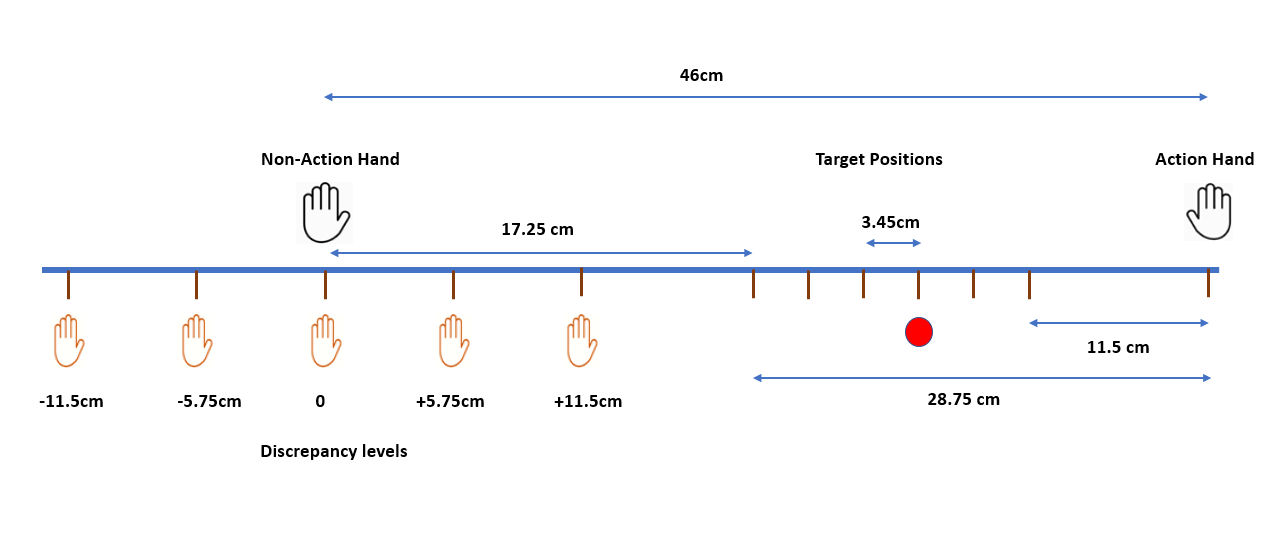
\includegraphics[width=\textwidth, keepaspectratio]{Images/exp2_task.png}
    \caption{Experimental Setup}
    \label{fig:exp2-task}
\end{figure}

Within each block, the target appeared at one of the following 6 locations along the axis joining the two docks, at a distance of  28.75, 25.30, 21.85, 18.40, 14.95, and 11.50 cm from the action hand (see Figure \ref{fig:exp2-task}). The experimental blocks each consisted of 10 x 6 (target positions) = 60 trials, while the filler blocks consisted of 5 trials each. 

The task performed by the participant was same as that of experiment 1. Each trial was initiated by bringing the right index finger on the right dock. On an audio cue, the target appeared at one of the above mentioned target locations, after which the participant attempted to make contact with the target with their right index position. The trial ended with the disappearance of the target after the contact was detected between the table and the right index finger. The participant brought the right hand back to the right dock to initiate the next trial. Throughout the course of the experiment, the right (action hand) was rendered invisible. 

\begin{table}[t]
\centering
\resizebox{\textwidth}{!}{
\begin{tabular}{llrr}
  \hline
  Model & Fixed effect & AIC & BIC \\
  \hline
  Null Model & None &	28746 &	28779 \\
  Discrepancy Model & Discrepancy	& 28731	& 28770 \\
  AHT Model & AHT &	28698 &	28737 \\
  Additive Model & Discrepancy + AHT	& 28683	& 28729 \\
  \textbf{Interaction Model} & \textbf{Discrepancy + AHT + (Discrepancy * AHT)} & \textbf{28666} & \textbf{28719}\\
   \hline
\end{tabular}}
\caption{AIC and BIC Values for fitted Linear Mixed Effect models. Random effects of all models consisted of intercepts for subjects and by-subject random slopes for effect of discrepancy ( $1 + discrepancy | subject$ ). The interaction model has the lowest AIC and BIC value. }
\label{table:lme-models}
\end{table}

  
 

\subsection{Experimental Design}

The accuracy of the spatial encoding of the target in reach action was operationalized as \textit{reach error}, which was computed as the difference between the actual location of the target and the estimated location of the target, indicated by the participant by the end-point of the reach action. Positive reach error indicates that the relative to the actual position of the target, the estimate of the target location is in the direction towards the action hand. On the other hand, negative reach error indicates that target location estimate is to the left of the actual target location in the direction of the the non-action hand. 

The experiment was set-up in a within-subjects experimental design, with reach error as the dependent variable. The two independent variables that were experimentally manipulated were - i) The non-action hand visuo-proprioceptive spatial discrepancy, that is, the distance between the actual position of the hand (proprioceptive hand) and the visual rendering of the hand (visual hand), and ii) The distance between the proprioceptive hand and target (PHT). 

\section{Results}
\begin{figure}[t]
\centering       
    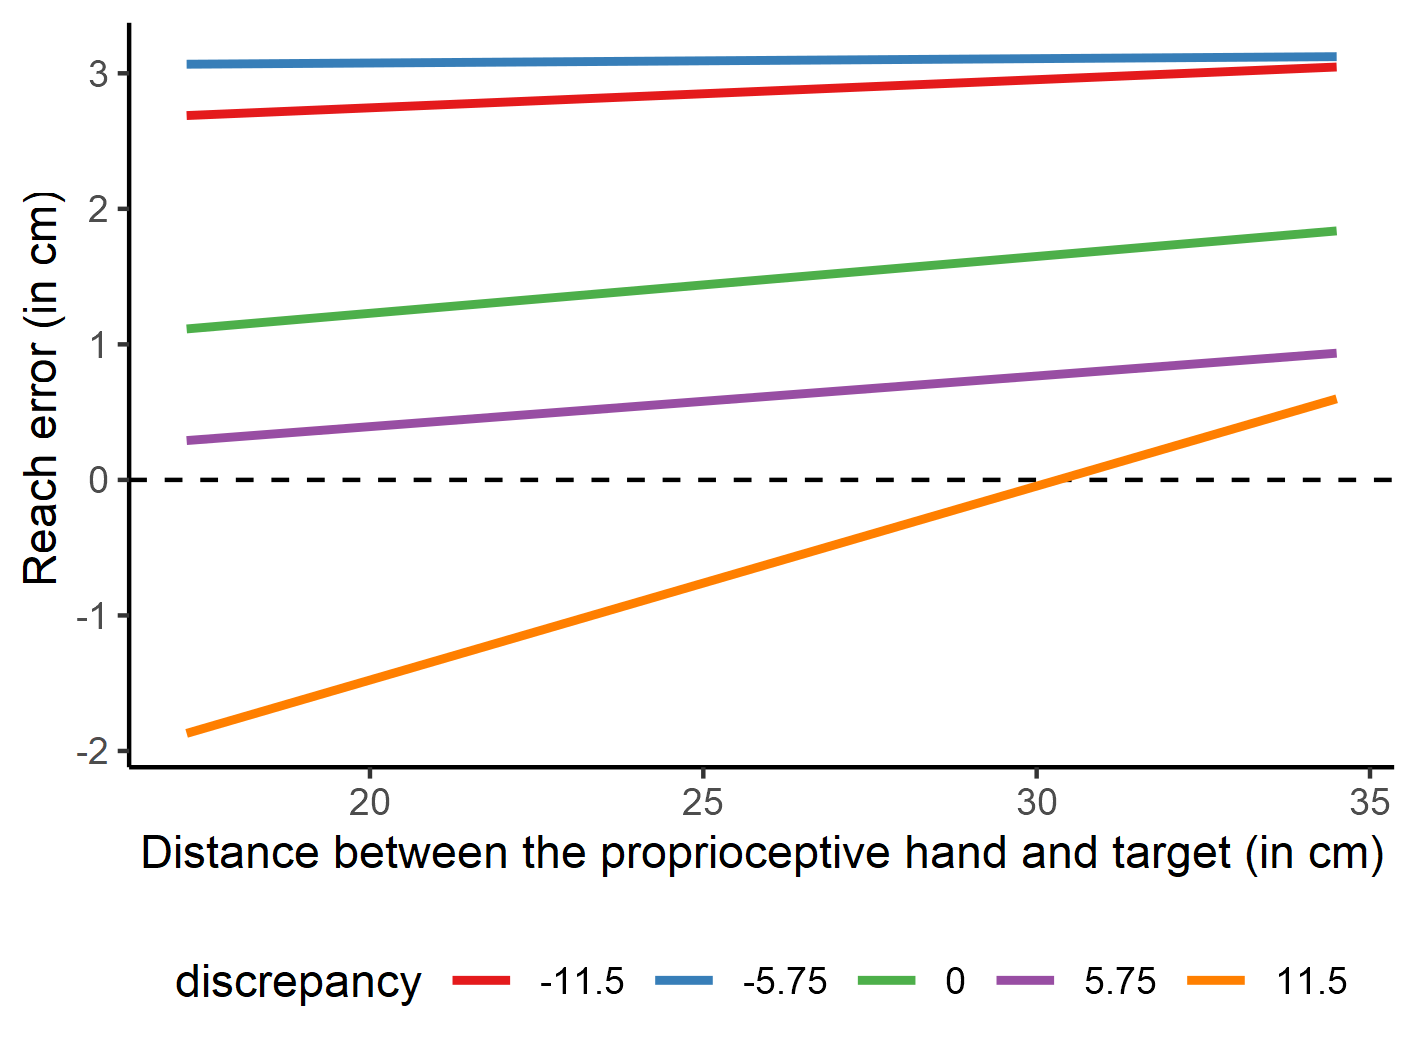
\includegraphics[scale=0.8]{Images/exp2_results.png}
    \caption{Reach error as a function of spatial discrepancy between the position of visual hand and the position of actual (proprioceptive) non-action hand. Each panel shows the distance between the target and the initial position of the action hand (AHT). Negative reach error indicates that the estimation of the target location was in the direction of the non-action hand towards the left, while positive reach error indicates that the location of the target was estimated in the direction of action hand towards the right of the actual location of the target.}
    \label{fig:exp2_re-pht}
\end{figure}

%\subsection{Data Analysis}

To understand the effect of visuo-proprioceptive spatial discrepancy and the distance from the target from the proprioceptive hand (PHT) on the reach error, we performed a linear mixed effects analysis using the \emph{lme4} ~\citep{bates2014fitting} and \emph{lmerTest} packages in R. Random effects of all models that we fit consisted of intercepts for the subjects and by-subject random slopes for the effect of discrepancy. Table \ref{table:lme-models} reports the AIC and BIC values of the models that we fit. Furthermore, we performed Likelihood Ratio Test to compare the models and as a criteria for model selection. Refer Appendix \ref{App-exp2-analysis} for the results of the Likelihood Ratio test. 

The AIC, BIC, and the results of the Likelihood Ratio Test reveal that the best fit model consisted of discrepancy and PHT as the fixed effects, along with an interaction between the two predictors. There were no obvious deviations from homoscedasticity and normality on the basis of visual inspection of residual plots. Furthermore, we checked for multi-collinearity between the predictors by using Variance Inflation Factor (VIF) as a measure of collinearity using the package \emph{performance} in R. The results show low correlation (VIF < 2) between the fixed effect terms of the best-fit model (see Table \ref{table:collinearity}).

Moreover, we performed bootstrapping to get credible confidence intervals at 95\% for the estimates of the fixed effects (see Table \ref{Table:Bootstrapped estimates}). None of the confidence intervals for the fixed effects contain the value 0, which further supports the significance of the effects of the three predictors (discrepancy, PHT, and interaction) on the reach error. 


\section{Discussion}
The results of the Linear Mixed Effects analysis shows that the interaction between the spatial discrepancy between the visual and proprioceptive inputs of the non-action hand and the distance between the target and the actual hand has a statistically significant effect on reach error. This suggests that the way visuo-proprioceptive spatial discrepancy of proximal non-action hand affects the target estimation depends upon the distance of the target from the the non-action hand. Figure \ref{fig:exp2_re-pht} shows the effect of proprioceptive hand and target distance (PHT) on reach error at different levels of discrepancy.

When the visual and the proprioceptive information provide congruent estimates for the location of the non-action hand (discrepancy = 0), the target location is underestimated towards the action hand. Reach accuracy is improved as the proximity between the target and the proprioceptive hand increases. As the visuo-proprioceptive discrepancy increases, with the visual hand being rendered closer to the target (discrepancy = +5.75cm), the reaches are more accurate. This suggests that the visual hand may be used as an anchor for the target representation due to its proximity to the target despite the discrepancy between the visual and proprioceptive inputs of the hand. However, as the discrepancy increases further, with visual hand moving even closer to the target (discrepancy = 11.5cm), the estimate of the target location is pulled towards the visual hand, as indicated by the negative values of the reach errors. This "pull" effect diminishes as the distance between the target and the proprioceptive hand increases. However, the close proximity of visual hand and target seems to increase the accuracy even though the visuo-proprioceptive discrepancy is high and when the target is far from the proprioceptive hand. In contrast, when the visuo-proprioceptive discrepancy is induced by rendering the visual hand away from the targets (discrepancy = -5.75cm and -11.50cm), overall high values of reach error are observed. The proximity between the proprioceptive hand and target do not have an effect on the reach error, in this case.

Overall, these results suggest that it is not merely the spatial discrepancy between the visual and proprioceptive information that affects the accuracy in target location estimation. Rather, the proximity of the visual hand to the target biases the estimation of the target in its direction, suggesting that the spatial encoding of the target may be anchored to the visual information of the body part in proximity.  

%These results contradict the hypothesis that of multi-sensory model to understand how target may be represented with respect to it. The model was that unisensory estimates will be combined to get a more reliable estimate. that means, the reliability will be more for the less discrepancy conditions and less for higher discrepancy conditions. There are thus two aspects, how reliable it is, and how close it is to the target. At negative discrepancy, 


 
\section{Bayesian Causal Inference Model}

To further interpret the results of the experiment, we qualitatively inspected the predictions of Bayesian Causal Inference Model and interpreted our results with respect to it. We find that there is no effect of distance from hand position predicted by the BCI model. On the other hand, the distance from the visual hand has a significant effect. 




































